\documentclass[12pt,oneside,letterpaper]{article}

\usepackage[canadien]{babel}
\usepackage[utf8]{inputenc}
\usepackage[T1]{fontenc}
\usepackage{lmodern}
\usepackage{graphicx}
\usepackage[letterpaper]{geometry}
\usepackage[americanvoltages,americancurrents, siunitx]{circuitikz}
\usetikzlibrary{babel}
\usepackage{caption}
\usepackage{subfig}
\usepackage{hyperref}
\usepackage[all]{hypcap}


\addto\captionsfrench{\def\tablename{Tableau}}
\captionsetup{font=small,labelfont=bf,margin=0.1\textwidth}
\pagestyle{myheadings}
\markboth{GPH-2006/PHY-2002~---~Composants~électriques~linéaires}{GPH-2006/PHY-2002~---~Composants~électriques~linéaires}


\begin{document}


\title{\textbf{Complément}\\Composants électriques linéaires}
\author{Jean-Raphaël Carrier \& Claudine Allen}
\date{}
\maketitle


\section{Introduction}

Un circuit électrique, aussi appelé réseau, est un ensemble de composants reliés par des fils conducteurs. Un courant électrique peut parcourir le circuit si ce dernier forme une (ou plusieurs) boucle fermée : on parle alors de circuit fermé. Il existe un très grand nombre de composants électriques différents ; seulement les principaux composants linéaires seront abordés dans ce complément (figure~\ref{circuit}).

\begin{figure}[h]
\begin{center}
\begin{circuitikz} \draw
(0,4) to[V, l_=$v_s$,*-*] (0,2) to[R,l_=$R_1$,*-*] (0,0) 
to[I,l_=$i_s$,*-*] (2,2) to[short,*-*] (0,2)
(0,4) to[L=$L$,*-*] (2,4)
(4,4) to[R,l_=$R_2$,*-*] (2,4) to[short,*-*] (2,2)
(4,2) node[ground]{} to[short,*-*] (4,4) 
(4,2) to[C, l_=$C$,*-*] (2,2)
{[anchor=east] (0,0) node {g} (0,2) node {d} (0,4) node {a}}
{[anchor=west] (4,4) node {c} (4,2) node {f}}
{[anchor=north west] (2,2) node {e}}
{[anchor=south] (2,4) node {b}}
;
\end{circuitikz}
\end{center}
\caption{\label{circuit}Circuit électrique composé d'une source de tension $v_s$, d'une source de courant $i_s$, de deux résistances $R_1$ et $R_2$, d'une bobine d'inductance $L$, d'un condensateur de capacité $C$ et d'une mise à la terre au n{\oe}ud $f$.}
\end{figure}

Chaque dipôle est doté de deux bornes, une borne positive ($+$) ainsi qu'une borne négative ($-$). Tous les composants mentionnés dans ce document sont des dipôles. La borne positive est toujours celle où le potentiel électrique est le plus élevé. Le sens positif du courant est défini (par convention, voir figure~\ref{xkcd}) comme étant la direction dans laquelle circuleraient des charges \textbf{positives}. Ainsi, le courant va du $+$ vers le $-$ ; il circule du potentiel le plus haut vers le potentiel le plus bas. Tous les dipôles sont complètement définis par la relation entre la différence de potentiel à leurs bornes et le courant qui les traverse.

Seules les sources d'alimentation font exception, puisqu'elles \textit{pompent} le courant : le courant à l'intérieur d'une source d'alimentation va donc du $-$ vers le $+$.

\begin{figure}[h]
\begin{center}
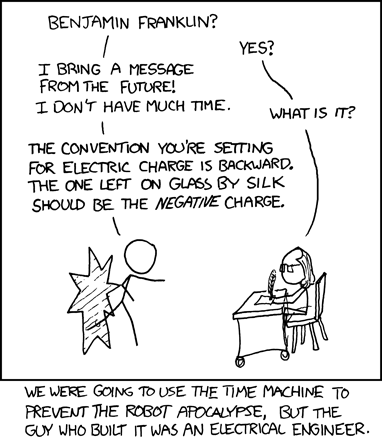
\includegraphics[width=0.5\textwidth]{xkcd-567}
\caption{\label{xkcd}Image pertinente (\texttt{www.xkcd.com/567/}).}
\end{center}
\end{figure}


\section{Sources d'alimentation}

Il existe deux types de sources d'alimentation : les sources de tension ($v_s$) et les sources de courant ($i_s$). Celles-ci fournissent respectivement une différence de potentiel (en volts) ou un courant (en ampères) dans un circuit électrique. En pratique, les sources de courant sont peu utilisées. Les sources d'alimentation peuvent être indépendantes ou commandées\footnote{Les plus sagaces auront remarqué qu'il existe alors quatre types de sources d'alimentation : de tension indépendante, de tension commandée, de courant indépendante et de courant commandée. L'auteur le sait et ne modifiera pas pour autant le troisième mot de cette section.}. La valeur de tension ou de courant fournie par une source indépendante n'est pas influencée par les autres composants du circuit. En d'autres mots, il y aura toujours 24~V aux bornes d'une source de tension indépendante de 24~V et il y aura toujours un courant de 50~mA qui circulera dans une source de courant indépendante de 50~mA, peu importe le circuit auquel elles sont rattachées. Quant à elle, une source commandée varie selon l'état d'un ou plusieurs composants du circuit. Par exemple, on pourrait utiliser une source de courant commandée pour injecter un courant qui serait en tout temps égal à la moitié du courant qui traverse une résistance donnée : la valeur du courant induit par cette source commandée serait donc directement fonction du circuit.

Il faut faire attention pour ne pas associer les termes \textit{indépendante} et \textit{commandée} à \textit{fixe} et \textit{ajustable}. Le bloc d'alimentation utilisé dans le cadre de ce cours est une source à la fois indépendante (pas fonction du circuit) et ajustable (l'utilisateur peut choisir la valeur de la source).

Dans un schéma, les sources d'alimentation indépendantes sont représentées par des cercles tandis que les sources commandées ont une forme de losange.

\begin{center}
\begin{circuitikz} \draw
(2,0) to[V, l_=$v_s$] (0,0)
(4,0) to[I=$i_s$] (6,0)
(10,0) to[cV, l_=$k \cdot v_x$] (8,0)
(12,0) to[cI=$k \cdot i_x$] (14,0)
;\end{circuitikz}
\end{center}

Les sources d'alimentation peuvent fournir un signal continu ou encore alternatif. Les sources sont des éléments \textit{actifs}, c'est-à-dire que la forme du signal dépendra d'elles. Les composants linéaires \textit{passifs} (résistances, bobines, condensateurs, etc.) adopteront le même comportement (continu ou alternatif) que la source. Ainsi, la tension et le courant pour tous les composants linéaires passifs reliés à une source sinusoïdale varieront aussi de façon sinusoïdale, et avec la même fréquence.


\section{Résistance}

La résistance est la capacité d'un élément à s'opposer au passage d'un courant électrique continu. La résistance, habituellement notée $R$, se mesure en ohms ($\Omega$). Le composant électrique associé à la résistance s'appelle aussi résistance (pour les distinguer, parfois le composant est appelé \textit{résisteur}). Une résistance ne peut pas accumuler de l'énergie ; elle ne fait qu'en dissiper par effet Joule (i.e. en chauffant).

\begin{center}
\begin{circuitikz} \draw
(0,0) to[R=$R$] (2,0)
;\end{circuitikz}
\end{center}

La relation entre la tension aux bornes d'une résistance et le courant qui la traverse est donnée par la loi d'Ohm:
\begin{equation}
\label{eq-loi-ohm}
v=R\,i.
\end{equation}


\section{Bobine d'inductance}

L'inductance, notée $L$, est la capacité d'un élément à s'opposer aux variations du courant qui le traverse. L'unité de l'inductance est le henry ($H$). Le composant électrique associé à cette grandeur est la bobine, aussi appelé solénoïde (ou tout simplement \textit{inductance} par abus de langage).

\begin{center}
\begin{circuitikz} \draw
(0,0) to[L=$L$] (2,0)
;\end{circuitikz}
\end{center}

Une bobine peut accumuler de l'énergie sous la forme d'un champ magnétique. Lorsqu'elle se vide, elle fournit de l'énergie au circuit : elle agit alors comme une source de courant. En courant continu, lorsqu'elle est pleinement chargée (régime permanent), la bobine agit comme un court-circuit (i.e. le courant circule librement).

Dans une bobine, la tension varie proportionnellement avec le taux de variation du courant:
\begin{equation}
\label{eq-tension-bobine}
v=L\,\frac{\mathrm{d}i}{\mathrm{d}t}.
\end{equation}


\section{Condensateur}

La capacité ($C$) est la grandeur qui caractérise l'opposition d'un élément vis-à-vis une variation de tension. Le composant s'appelle un condensateur et l'unité est le farad ($F$).

\begin{center}
\begin{circuitikz} \draw
(0,0) to[C=$C$] (2,0)
;\end{circuitikz}
\end{center}

Un condensateur peut accumuler de l'énergie sous la forme d'un champ électrique. Lorsqu'il se vide, il fournit de l'énergie au circuit : il agit alors comme une source de tension. En courant continu, lorsqu'il est pleinement chargé (régime permanent), le condensateur agit comme un circuit ouvert (i.e. aucun courant n'y circule).

La tension aux bornes du condensateur est proportionnelle à la charge électrique qui y est accumulée:
\begin{equation}
\label{eq-tension-condensateur-1}
v=\frac{q}{C}.
\end{equation}
Or, par définition, le courant est donné par le taux de varation de la charge:
\begin{equation}
\label{eq-courant}
i=\frac{\mathrm{d}q}{\mathrm{d}t}.
\end{equation}
En combinant les équations \ref{eq-tension-condensateur-1} et \ref{eq-courant} on obtient:
\begin{equation}
\label{eq-tension-condensateur-2}
v=\frac{1}{C}\,\int i\,\mathrm{d}t.
\end{equation}


\section{Mise à la terre}

En électricité, on parle de \textit{différence de potentiel} et non directement de \textit{potentiel}. En d'autres mots, une référence est toujours nécessaire. Par analogie, si vous voulez caractériser la hauteur\footnote{Ici «hauteur» doit être compris dans le sens «altitude».} de votre crayon, vous devez spécifier à partir de quelle référence votre mesure est prise (ex: la table, le sol, le niveau de la mer...). En électricité, la référence la plus générale est le potentiel du sol. Le sol a par convention un potentiel invariable nul. Un n{\oe}ud peut être mis au potentiel du sol à l'aide d'une mise à la terre (\textit{ground}), aussi appelée mise à la masse.

\begin{center}
\begin{circuitikz} \draw
(0,0) node[ground]{}
;\end{circuitikz}
\end{center}

De façon opposée, une différence de potentiel n'a pas besoin de référentiel puisqu'elle compare directement deux points (les bornes d'une résistance, par exemple). Pour les mêmes raisons, vous n'avez pas besoin de référence pour mesurer la longueur de votre crayon : celle-ci aura la même valeur que vous soyez sur la Lune ou dans les tréfonds de l'Enfer.


\end{document}

Écrit par Jean-Raphaël Carrier
Dernière modification : 10 janvier 2014